\documentclass{article}

\usepackage{amsmath}
\usepackage{amssymb}
\usepackage{graphicx}

\begin{document}


Ivan Lin\newline{}
Dr. Esther Arkin\newline{}
AMS301\newline{}
3/3/17

\begin{center}
  Homework 5a
\end{center}

\underline{Problem A}
Let $T$ be a balanced 5-ary tree with 81 nodes.\newline{}
(a). How many internal nodes does T have?\newline{}
(b). How many edges does the tree T have?\newline{}
(c). What is the height of T?\newline{}

(a). Using the equation $n=mi+1$ where $n$ is the number of nodes, $i$ is the number of internal nodes, and $m$ is the number of child nodes for each parent, we can plug in and determine the answer is $i=16$ internal nodes.

(b). Since a tree with $n$ nodes has $n-1$ edges, we can determine that $T$ has 80 edges.

(c). The height of the tree from the root is determined by $1+log_m(n)$, in this case $2 < log_5(81) < 3$. This rounds up to 3, meaning there are $4$ levels including the root.

\underline{Section 3.1 Problem 2}

Suppose a connected graph has 20 edges. What is the maximum possible number
of vertices?

In order to maximize the number of vertices, the graph should be minimally connected without circuits in order to prevent redundancy. Trees are example of such graphs, which have the property there is one fewer edge than there are nodes. This means that if the connected graph has $20$ edges, there would be $21$ vertices.

\underline{Section 3.1 Problem 16}

Given $G$, an $n$ vertex forest of $t$ trees we can find the number of edges in the graph. Any subtree can be formed from a larger tree by taking away any edge, since trees are minimally connected. A tree with $n$ vertices would have $n-1$ edges. $t$ disjoint subtrees can be formed by taking away $t-1$ edges. Therefore, the graph $G$ will have $(n-1)-(t-1)$ or $n-t$ subtrees.

\underline{Section 3.1 Problem 28}

Find the minimum amount of weighings to find the any differently weighed coins out of 20, where at most one coin is too light.

It would take three weighings to find the lighter coin if one exists.

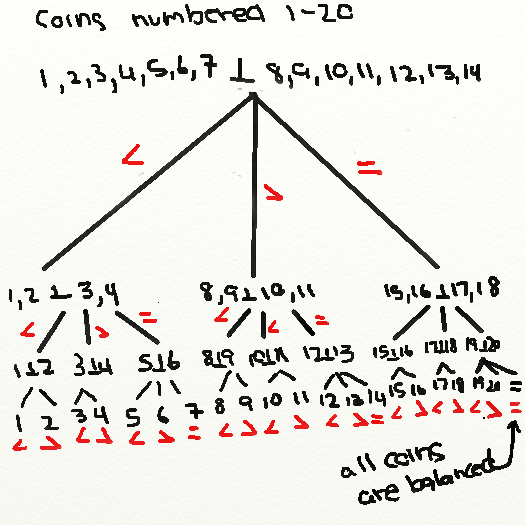
\includegraphics[width=\textwidth]{s3-1p28.png}

\end{document}
